\chapter{Lossless and Low-Loss Transmission Line}\label{lec:lec4}
\section{Matched Condition of the transmission line}
From the previous chapter, we got that
\begin{align*}
\Gamma_L \equiv \Gamma{(0)} = \frac{Z_L - Z_0}{Z_L + Z_0}
\end{align*}
Where $\Gamma_L$ is the reflection coefficient at the load end. $\Gamma_L$ is a measure of how much energy is reflected from the load end and is related to the terminating impedance of the line and the characteristics impedance:\\

Therefore, 
\begin{align*}
\Gamma_L = \frac{Z_L - Z_0}{Z_L + Z_0} =  \frac{V^-}{V^+}
\end{align*}
Which is the reflection co-efficient at load point when $l = 0$.\\\\
We see immediately that when  $Z_L = Z_0$, then there is no reflection from the load and hence maximum power is delivered to the generator.
\begin{align*}
\Gamma_L = \frac{V^-}{V^+} = 0\ (\text{when }Z_L = Z_0.) 
\end{align*}
Although $Z_0$ cannot be located on the transmission line, it does govern power flow in the transmission line. This condition that $Z_L = Z_0$ is called the \textbf{Matched condition} of the transmission line. The terminating impedance of the line is matched to the characteristic impedance. This condition is similar to the maximum power transfer theorem in a circuit, where if the load impedance is equal to the conjugate of the generator impedance, maximum power is transferred from the generator to the load. 
\begin{align*}
Z_L = Z_0 \quad (\text{Matched Load Condition})
\end{align*}
As the wave moves along the line, it sees $Z_0$. At $Z_L$, it suddenly sees an impedance discontinuity from $Z_0$ to $Z_L$ which is like a steep change because of that part of the energy that tends to get reflected by the generator on the transmission line. So, for maximum power transfer, the terminating load impedance must be equal to the characteristics impedance; otherwise, maximum power transfer will not take place and there will always be reflection.\\

The reflection Co-efficient at any point on the transmission line is given as:
\begin{align*}
\Gamma{(l)} = \frac{V^-e^{-\gamma l}}{V^+e^{\gamma l}} = \frac{\text{Backward wave}}{\text{Forward wave}}
\end{align*}
Therefore we can define the voltage and current at any point on the transmission line with respect to reflection coefficient $\Gamma(l)$.
\begin{equation}
V(l) = V^+e^{\gamma l} + V^-e^{-\gamma l}
\end{equation}
\begin{equation}
I(l) =\frac{V^+}{Z_0} e^{\gamma l} - \frac{V^-}{Z_0}e^{-\gamma l}
\end{equation}\\\\
Dividing Equation 4.1 by $V^+e^{\gamma l}$
\begin{align*}
\frac{V(l)}{ V^+e^{\gamma l}} = 1 + \frac{ V^-e^{-\gamma l}}{ V^+e^{\gamma l}}
\end{align*}
\begin{align*}
\frac{V(l)}{ V^+e^{\gamma l}} = 1 + \Gamma(l)
\end{align*}
We then cross-multiply to have
\begin{align*}
V(l) = V^+e^{\gamma l} (1 + \Gamma(l))
\end{align*}
The above equation gives the voltage at any point on the line\\
Divide Equation 4.2 by $\frac{V^+}{Z_0} e^{\gamma l}$
\begin{align*}
\frac{I}{\frac{V^+}{Z_0} e^{\gamma l}} = 1 - \frac{\frac{V^-}{Z_0} e^{-\gamma l}}{\frac{V^+}{Z_0} e^{\gamma l}}
\end{align*}
\begin{align*}
\frac{I}{\frac{V^+}{Z_0} e^{\gamma l}}= 1 - \frac{V^-e^{-\gamma l}}{V^+e^{\gamma l}}
\end{align*}
\begin{align*}
\frac{I}{\frac{V^+}{Z_0} e^{\gamma l}} = 1 - \Gamma(l)
\end{align*}
We cross-multiply again to get,
\begin{align*}
I(l) = \frac{V^+}{Z_0} e^{\gamma l} (1 - \Gamma(l))
\end{align*}
Where $Z(l) = \frac{V(l)}{I(l)}$, we have
\begin{align*}
Z(l) = \frac{V(l)}{I(l)} = \frac{V^+e^{\gamma l} (1 + \Gamma(l))}{ \frac{V^+}{Z_0} e^{\gamma l} (1 - \Gamma(l))}
\end{align*}
$V^+ e^{\gamma l}$ cancels out to give,
\begin{align}
Z(l) = Z_0[\frac{1 + \Gamma(l)}{1 - \Gamma(l)}]
\end{align}

$Z(l)$ is the impedance measured at any location of the transmission line. It is related to the reflection coefficient at any point and the characteristic impedance.
$\Gamma(l)$ is the reflection coefficient at any point on the transmission line.
Hence $Z(l)$ and $\Gamma(l)$ have a one-to-one relationship at any point along the transmission line.\\\\
\section{Impedance Transform Relationship}
Recall,
\begin{align*}
Z(l) = \frac{V(l)}{I(l)}
\end{align*}
\begin{align*}
Z(l) = \frac{V^+e^{\gamma l} + V^-e^{-\gamma l}}{\frac{V^+}{Z_0}e^{\gamma l} - \frac{V^-}{Z_0}e^{-\gamma l}}
\end{align*}
\begin{align*}
Z(l) = Z_0[\frac{V^+e^{\gamma l} + V^-e^{-\gamma l}}{V^+e^{\gamma l} - V^-e^{-\gamma l}}]
\end{align*}
Dividing  the numerator and denominator by $V^+e^{\gamma l}$ 
\begin{align*}
Z(l) = Z_0[\frac{1 + \frac{V^-e^{-\gamma l}}{V^+e^{\gamma l}}}{1 - \frac{V^-e^{-\gamma }}{V^+e^{\gamma }}}]
\end{align*}
Where $\Gamma_L = \frac{V^-}{V^+}$ and $\frac{e^{-\gamma l}}{e^{\gamma l}} = e^{-2\gamma l}$
\begin{align}
Z(l)=  Z_0\left[\frac{1 + \Gamma_L e^{-2\gamma l}}{1 - \Gamma_L e^{-2\gamma l}}\right]
\end{align}
But $\Gamma_L
= \frac{Z_L - Z_0}{Z_L + Z_0}$,
\begin{align*}
Z(l) = Z_0 \left[\frac{1 + (\frac{Z_L - Z_0}{Z_L + Z_0})e^{-2\gamma l}}{1 - (\frac{Z_L - Z_0}{Z_L + Z_0})e^{-2\gamma l}}\right]
\end{align*}
Multiplying the numerator and denominator by $Z_L + Z_0 $\\
which gives
\begin{align*}
Z(l) = Z_0 \left[\frac{(Z_L + Z_0) + (Z_L - Z_0)e^{-2\gamma l}}{(Z_L + Z_0) - (Z_L - Z_0)e^{-2\gamma l}}\right]
\end{align*}
\begin{align*}
Z(l) = Z_0 \frac{e^{-\gamma l}}{e^{-\gamma l}}\left[\frac{(Z_L + Z_0)e^{\gamma l} + (Z_L - Z_0)e^{-\gamma l}}{(Z_L + Z_0)e^{\gamma l} - (Z_L - Z_0)e^{-\gamma l}}\right]
\end{align*}
$e^{-\gamma l}$ cancels out, and we open the bracket
\begin{align*}
Z(l) = Z_0 \left[\frac{Z_Le^{\gamma l} + Z_0e^{\gamma l} + Z_Le^{-\gamma l} - Z_0e^{-\gamma l}}{Z_L e^{\gamma l} + Z_0e^{\gamma l} - Z_Le^{-\gamma l} + Z_0e^{-\gamma l}}\right]
\end{align*}
Collect like terms
\begin{align*}
Z(l) = Z_0 \left[\frac{Z_L(e^{\gamma l} + e^{-\gamma l}) + Z_0(e^{\gamma l} - e^{-\gamma l})}{Z_L (e^{\gamma l} - e^{-\gamma l}) + Z_0(e^{\gamma l} + e^{-\gamma l})}\right]
\end{align*}
Recall; 
\begin{align*}
cosh\gamma l = \frac{e^{\gamma l} + e^{-\gamma l}}{2}\\
2cosh\gamma l = e^{\gamma l} + e^{\gamma l}
\end{align*}
\begin{align*}
sinh\gamma l = \frac{e^{\gamma l} - e^{-\gamma l}}{2}\\
2sinh\gamma l = e^{\gamma l} - e^{-\gamma l}
\end{align*}
Therefore,
\begin{align*}
Z(l) = Z_0\left[\frac{2(Z_Lcosh\gamma l + Z_0sinh\gamma l)}{2(Z_Lsinh\gamma l + Z_0cosh\gamma l)}\right]
\end{align*}
\begin{align}
Z(l) = Z_0\left[\frac{Z_Lcosh\gamma l + Z_0sinh\gamma l}{Z_Lsinh\gamma l + Z_0cosh\gamma l}\right]
\label{eqn:imp}
\end{align}
The impedance at any point $l$ is related to the load impedance $Z_L$ and the characteristics impedance $Z_0$ by the above relationship. This enables us to move $Z_L$ to any point along the transmission line. Hence at $l = 0$, we have $Z_L$ but at $l = L$, the input impedance measured at the generator end will not be $Z_L$. It will depend on $Z_L$ and also the length of the line. So, if the length of the line keeps varying, the impedance you measure at the input end of the line will keep varying. 

Hence, if we design a circuit at high frequency and connect a load to the end, depending on the length of the transmission line, the input impedance will keep varying with length. From a circuit perspective, the input impedance is very important. So at high frequencies, the length connecting the load to the circuit matters as the input impedance seen by the generator varies with length.\\\\
From Equation \ref{eqn:imp}:
\begin{align*}
Z(l) = Z_0\left[\frac{Z_Lcosh\gamma l + Z_0sinh\gamma l}{Z_Lsinh\gamma l + Z_0cosh\gamma l}\right]
\end{align*}
Now normalized with respect to $Z_0$ such that if,
$\frac{Z(l)}{Z_0} = \bar{Z}(l)$ and $\frac{Z_L}{Z_0} =\bar{Z}_L$ that is, normalized values.\\\\
Therefore, dividing both sides by $Z_0$
\begin{align*}
\frac{Z(l)}{Z_0} = \frac{Z_0}{Z_0}[\frac{Z_Lcosh\gamma l + Z_0sinh\gamma l}{Z_Lsinh\gamma l + Z_0cosh\gamma l}] 
\end{align*}
Divide Numerator and Denominator by $Z_0$
\begin{align*}
\bar{Z}(l) =\left [ \frac{\frac{Z_L}{Z_0}cosh\gamma l + \frac{Z_0}{Z_0}sinh\gamma l}{\frac{Z_L}{Z_0}sinh\gamma l + \frac{Z_0}{Z_0}cosh\gamma l}\right]
\end{align*}
\begin{align*}
\bar{Z}(l) = \frac{\frac{Z_L}{Z_0}cosh\gamma l + sinh\gamma l}{\frac{Z_L}{Z_0}sinh\gamma l + cosh\gamma l}
\end{align*}
\begin{align}
\bar{Z}(l) = \frac{\bar{Z}_Lcosh\gamma l + sinh\gamma l}{\bar{Z}_Lsinh\gamma l + cosh\gamma l}\ \text{(normalized impedance)}
\end{align} 
That is, $\bar{Z} = \frac{Z}{Z_0}$ .
Once again we see that on transmission line calculation, the absolute impedance does not mean anything; Rather it is the normalized impedance that matters most. Hence, $Z_0 = 50\Omega$ and $Z_L = 100\Omega$ gives same reflection as $Z_0 = 300\Omega$ and $Z_L =600\Omega$. Hence the reason why before starting any transmission line calculation, we ask ourselves what the characteristic impedance is, every impedance we have is then normalized to the characteristic impedance. So every calculation done in the transmission line is always done with respect to normalized impedances.\\
We then see that characteristic impedance which is not located anywhere or seen anywhere is always governing the energy flow of the transmission line.\\
Now if $\bar{Z}_L = 1$, then 
\begin{align*}
\bar{Z}(l) = {\frac{\bar{Z}_Lcosh\gamma l + sinh\gamma l}{\bar{Z}_Lsinh\gamma l + cosh\gamma l}} = 1
\end{align*}
Recall: $\frac{Z(l)}{Z_0} = \bar{Z}(l)$ and $\frac{Z_L}{Z_0} = \bar{Z}_L$\\
\begin{align*}
\frac{Z(l)}{Z_0} = 1,\frac{Z_L}{Z_0} = 1
\end{align*}
That means impedance at every point = $Z_0$ if $Z_L = Z_0$ therefore $Z(l) = Z_0$. So, in this matched condition, the impedance $Z(l)$ measured at any point no longer depend on the length of the line. So if a line is terminated by its characteristic impedance, there is no need to bother about the length of the line as every point along the line has an impedance equal to the characteristic impedance and this takes away all the worry about the line length.
The relationship of impedance transform will help us give a proper definition of characteristics impedance $Z_0$ which we know was related to the primary constants of the transmission line.
\section{Characteristic Impedance}  
Characteristic Impedance is defined as the impedance which is used to terminate the line, the impedance measured at all points along the line will be the same and equal to that terminating impedance.

At matched conditions, there is no reflected wave. With infinite line length, there can be no reflection as the incident wave never gets to the end to get reflected. Hence, the reflection is zero. However, reflection is zero when the line is terminated with the characteristic impedance. Hence, the characteristic impedance can also be defined as the input impedance measured with infinite line length; since with infinite line length, we always have a forward wave and never a reflected wave.\\\\
Now we can generalize the impedance transformation relationship. Till now, we have transformed impedance $Z_L$ which is at the load end to $Z(l)$. Nothing special about the load end other than we defining our origin to be at that point. So, the load point was used as our reference point. In general, look at the transmission line below:
\begin{figure}[h]
\centering
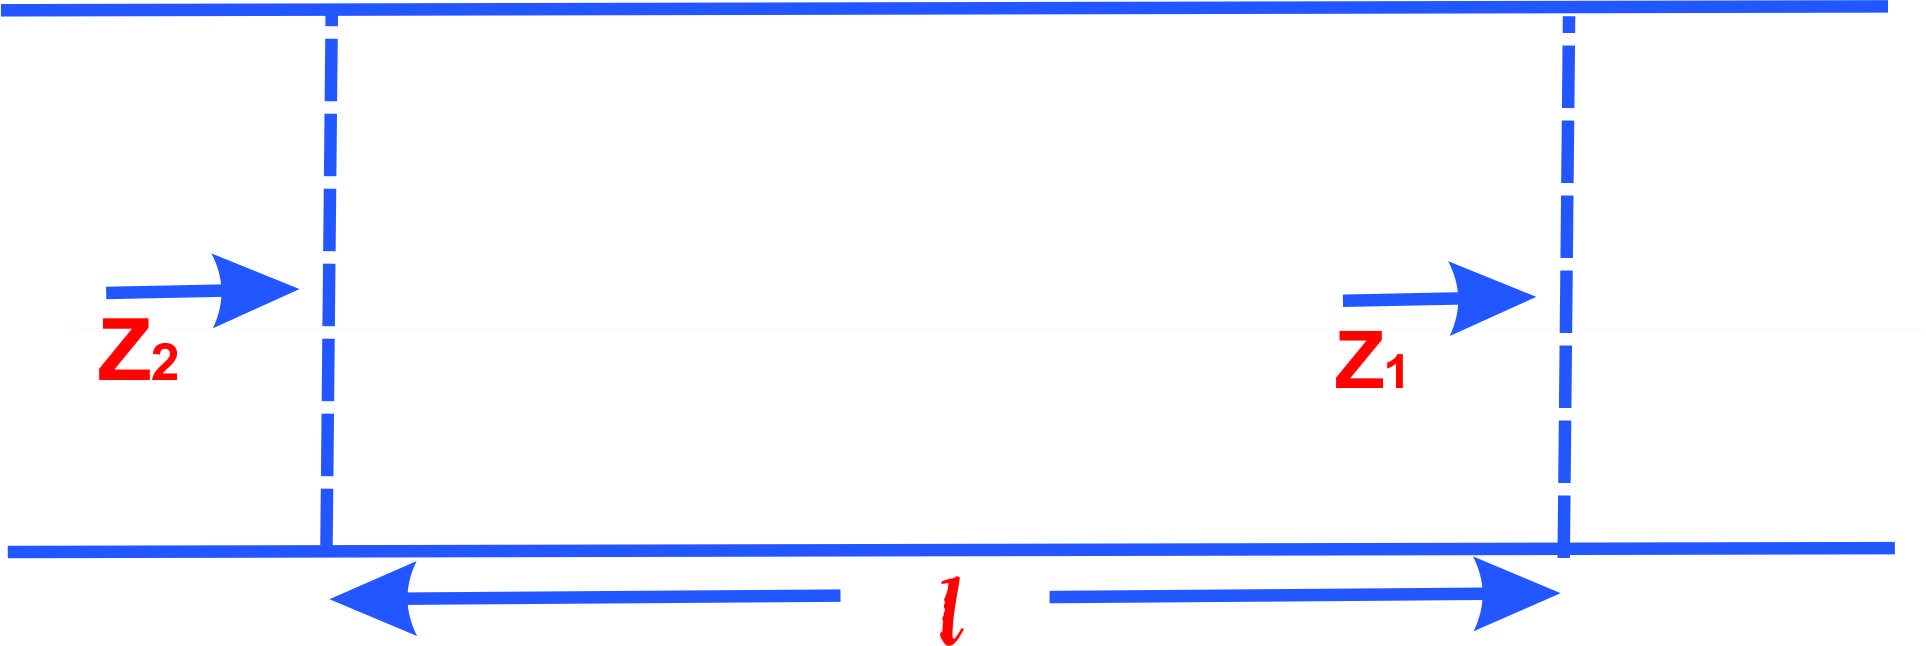
\includegraphics[scale=0.45]{./graphics/1234}
\caption{}
\end{figure}

recall from Equation 4.5: 
\begin{align*}
Z(l) = Z_0\left[\frac{Z_Lcosh\gamma l + Z_0sinh\gamma l}{Z_Lsinh\gamma l + Z_0cosh\gamma l}\right]
\end{align*}
Here, $Z_L = Z_1$ and $Z(l) = Z_2$.\\
\begin{align}
Z_2 = Z_0\left[\frac{Z_1cosh\gamma l + Z_0sinh\gamma l}{Z_1 sinh\gamma l + Z_0 cosh\gamma l}\right]
\label{eqn:z2norm}
\end{align}
Dividing both sides by $Z_0$
\begin{align*}
\frac{Z_2}{Z_0} = \frac{Z_0}{Z_0} \left[\frac{Z_1cosh\gamma l + Z_0sinh\gamma l}{Z_1 sinh\gamma l + Z_0 cosh\gamma l}\right]
\end{align*}
Divide the numerator and denominator by $Z_0$
\begin{align*}
\frac{Z_2}{Z_0} = \left[\frac{\frac{Z_1}{Z_0}cosh\gamma l + \frac{Z_0}{Z_0}sinh\gamma l}{\frac{Z_1}{Z_0}sinh\gamma l + \frac{Z_0}{Z_0}cosh\gamma l}\right]
\end{align*}
\begin{align*}
\bar{Z}_2 = \left[\frac{\frac{Z_1}{Z_0}cosh\gamma l + sinh\gamma l}{\frac{Z_1}{Z_0}sinh\gamma l + cosh\gamma l}\right]
\end{align*}
\begin{align*}
\bar{Z}_2 = \left[\frac{\bar{Z}_1cosh\gamma l + sinh\gamma l}{\bar{Z}_1sinh\gamma l + cosh\gamma l}\right]
\end{align*}
From Equation~\ref{eqn:z2norm} we can also invert the relationship to get $Z_1$ from $Z_2$ by cross multiplying.
\begin{align*}
Z_2 = Z_0\left[\frac{Z_1cosh\gamma l + Z_0sinh\gamma l}{Z_1 sinh\gamma l + Z_0 cosh\gamma l}\right]
\end{align*}
\begin{align*}
Z_2[Z_1sinh\gamma l + Z_0cosh\gamma l] = Z_0[Z_1cosh\gamma l + Z_0sinh\gamma l]
\end{align*}
$Z_1Z_2sinh\gamma l + Z_0Z_2cosh\gamma l = Z_0Z_1cosh\gamma l + Z_0^2sinh\gamma l$\\\\
Collect like terms and factorise out $Z_1$ on the left and $Z_0$ on the right-hand side of the equation
\begin{align*}
Z_1Z_2sinh\gamma l - Z_1Z_0cosh\gamma l = Z_0^2sinh\gamma l - Z_0Z_2cosh\gamma l]
\end{align*}
\begin{align*}
Z_1[Z_2sinh\gamma l - Z_0cosh\gamma l] = Z_0[Z_0sinh\gamma l - Z_2cosh\gamma l]
\end{align*}
Make $Z_1$ the subject of the formula
\begin{align}
Z_1 = Z_0\left[\frac{Z_0sinh\gamma l - Z_2cosh\gamma l}{Z_2sinh\gamma l - Z_0cosh\gamma l}\right]
\label{eqn:z2norminv}
\end{align}
Multiply the numerator and denominator of Equation~\ref{eqn:z2norminv} by $-1$.
\begin{align*}
Z_1 = Z_0\left[\frac{Z_2cosh\gamma l - Z_0sinh\gamma l}{Z_0cosh\gamma l - Z_2sinh\gamma l}\right]
\end{align*}
Recall:
\begin{align*}
cosh\gamma l = cosh(-\gamma l)
\end{align*}
\begin{align*}
sinh\gamma l = -sinh(-\gamma l)
\end{align*}
So that,
\begin{align*}
sinh(-\gamma l) = -sinh\gamma l
\end{align*}
So, equation~\ref{eqn:imp} can be used to transform impedance between $Z_1$ and $Z_2$ knowing the positive $l$ direction is from load towards the generator.\\\\
Now we go to a special case of the transmission lines.

\section{Lossless Transmission Line}

In practice, we want to transfer maximum power from the generator to the load. However, some losses occur in real transmission lines due to ohmic resistances. Every effort is usually made to make sure maximum power is delivered to the load by minimizing their losses. Hence, a good transmission line loss should be very small at its operating frequency. 

Once we have this condition in practice, then we can make some simplification to the transmission line problem and come up with an idea of what is called a \textbf{lossless transmission line}; whose ideal loss is zero.

The transmission line has four parameters $R, L, G$ and $C$ all in per unit length. $R$ and $G$ are ohmic values in the primary constant, that is, the resistance between the two ends of the conductors and the leakage current in the dielectric separating the two conductors respectively. Hence, power-losing elements exist because of the resistance and conductance. The inductance and capacitance exchange energy between themselves but does not result in any loss. Ideally, a line will be lossless if $R = G = 0$.\\

Substituting $R$ and $G$ as Zero in the Telegrapher's equation.
\begin{align*}
\gamma = \sqrt{(R + \jmath\omega L)(G + \jmath\omega C)}
\end{align*}
\begin{align*}
= \sqrt{(\jmath\omega L)(\jmath\omega C)}
\end{align*}
\begin{align*}
\gamma = \jmath\omega\sqrt{LC}
\end{align*}
Also,
\begin{align*}
\gamma = \alpha + \jmath\beta
\end{align*} 
Therefore,
\begin{align*}
\alpha + j\beta = \jmath\omega\sqrt{LC}
\end{align*}
so,
\begin{align*}
\alpha = 0, \beta = \omega\sqrt{LC}
\end{align*}

With no loss, there is no reason for the wave amplitude to reduce on the transmission line since $\alpha = 0$(The Attenuation Constant). Hence, there is a sustained propagation of electromagnetic waves along the transmission line.\\
$\beta = \omega\sqrt{LC}$ but $\beta = \frac{2\pi}{\lambda}$ and $\omega = 2\pi f $. That is,
\begin{align*}
\frac{2\pi}{\lambda} = 2\pi f\sqrt{LC}
\end{align*}
$2\pi$ will cancel out to give,
\begin{align*}
\frac{1}{\lambda} =  f\sqrt{LC}
\end{align*}
Recall, $\lambda f = V$ which is the velocity of the wave in the transmission line.
\begin{align*}
\lambda f = \frac{1}{\sqrt{LC}} = V
\end{align*}
The velocity of the wave in the transmission line is related to the inductance and capacitance of the transmission line. Hence the velocity is fixed once the inductance and capacitance are given.

Can we vary load $L$ and $C$ to vary $V$? Not really, $L$ and $C$ are coupled. Varying $C$ changes $L$ and varying $L$ changes $C$ to make $V$ a constant of the transmission line. The velocity parameter is decided by the field condition in the transmission line and is fixed by the boundary condition. 

For instance, with varying separation between the two conductors, the mutual inductance will vary and at the same time, the separation between the two conductors vary thereby varying the capacitance. Hence, $L$ and $C$ of the transmission line are not independent quantities.\\
We then calculate the characteristic impedance on a lossless transmission line which is given as,
\begin{align*}
Z_0 = \sqrt{\frac{R + \jmath\omega L}{G + \jmath\omega C}} = \sqrt{\frac{\jmath\omega L}{\jmath\omega C}} = \sqrt{\frac{L}{C}}.
\end{align*}
Which is a real quantity. So, for a lossless line, $Z_0$ is REAL. We do not have any ohmic resistance or conductance in the line and yet it is at this point we have a characteristic impedance that is real. That is, Pure ohmic. Hence, the wave which travels forward or backwards always sees a characteristic impedance that is a real impedance like resistance. This makes sense since you have a line carrying only forward waves which will go forever and no energy is reflected. 

That is, power somewhere is going to get dumped. So if we have a real quantity for $Z_0$, it means that power is completely transferred to the line; it does not mean that power is lost in the line. So for a lossless line, if the impedance on the line is measured, something more like resistance will be measured.

Now, we go to a case where little loss is accepted in the transmission line and then find the derivations for $\gamma$ and $Z_0$.
\section{Low-loss Transmission Line}
$R \ll \omega L$, $G \ll \omega C$ are the two conditions for a low-loss transmission line. Using the Telegrapher's equation, we have:
\begin{align*}
\gamma = \sqrt{(R + \jmath\omega L)(G + \jmath\omega C)}
\end{align*}
Which is the same as,
\begin{align*}
\gamma = \sqrt{{(\jmath\omega L)(\jmath\omega C)(1 + \frac{R}{\jmath\omega L})(1 + \frac{G}{\jmath\omega C})}}
\end{align*}
where $\frac{1}{\jmath} = -\jmath$, we have that $\gamma$ is
\begin{align*}
= \sqrt{{(\jmath\omega L)(\jmath\omega C)(1 - j\frac{R}{\omega L})(1 - j\frac{G}{\omega C})}}
\end{align*}
Recall from Binomial expansion with fraction power\\\\
$(1 + x)^{\frac{1}{2}} = \frac{1}{2}C_0(1)^{\frac{1}{2}}x^0 + \frac{1}{2}C_1(1)^{{\frac{1}{2}} - 1}x^1 + ...$\\\\
$\frac{1}{2}C_0(1)^{\frac{1}{2}}x^0 = 1$\\\\
$\frac{1}{2}C_1(1)^{\frac{1}{2} - 1}x = \frac{1}{2}C_1(1)x$\\\\
Note that 1 to the power of any value is 1 provided it is not infinity.\\\\
$\frac{1}{2}C_1 = \frac{\frac{1}{2}x!}{(x - 1)!1!} = \frac{\frac{1}{2}x(x-1)!}{(x-1)!1!} = \frac{1}{2}x$\\\\
$n! = n(n - 1)!$\\\\
$(1 + x)^{\frac{1}{2}} = 1 + \frac{1}{2}x + .....$\\\\
$(1 - x)^{\frac{1}{2}} = 1 - \frac{1}{2}x + .....$\\\\
Hence from the equation
$jw\sqrt{LC}(1 - \frac{\jmath R}{wL})^{\frac{1}{2}}(1 - \frac{\jmath G}{wC})^{\frac{1}{2}}$\\\\
Let $x = \frac{\jmath R}{\omega L}$ and $x' = \frac{\jmath G}{\omega C}$\\\\
$(1 - \frac{\jmath R}{\omega L})^{\frac{1}{2}} =[1 - \frac{1}{2}\frac{\jmath G}{\omega C} + ....]$\\\\
$(1 - \frac{jG}{\omega C})^{\frac{1}{2}} =[1 - \frac{1}{2}\frac{\jmath R}{\omega L} + ....]$\\\\
$= jw\sqrt{LC}(1 - \jmath \frac{R}{2\omega L} + ...)(1 - j\frac{G}{2\omega C} + ...)$\\\\
$= jw\sqrt{LC} [1- [\frac{\jmath R}{2\omega L}] - [\frac{\jmath G}{2\omega C}] + [\frac{\jmath R}{2\omega L}][\frac{\jmath G}{2\omega C}]]$\\\\
Recall that two combination terms were used earlier because of the complex variable $\frac{jR}{wL}$ and $\frac{\jmath G}{\omega C}$, the product of $\frac{\jmath R}{2\omega C}$ and $\frac{\jmath G}{2\omega L}$ tends to zero since $R \ll wL$ and $G \ll \omega C$ for a low loss transmission line.\\\\
$= \jmath\omega\sqrt{LC} [1- [\frac{\jmath R}{2\omega L}] - [\frac{\jmath G}{2\omega C}]]$\\\\
Expanding we have,
\begin{align*}
= \jmath\omega\sqrt{LC} - \jmath\frac{R}{2\omega L}(\jmath\omega\sqrt{LC}) - j\frac{G}{2\omega C}(\jmath\omega\sqrt{LC})
\end{align*}
Where L = $\sqrt{L} \times \sqrt{L}$ and C = $\sqrt{C} \times \sqrt{C}$, we have
\begin{align*}
= \jmath\omega\sqrt{LC} + \frac{R\sqrt{L}\sqrt{C}}{2\sqrt{L}\sqrt{L}} + \frac{G\sqrt{L}\sqrt{C}}{2\sqrt{C}\sqrt{C}}
\end{align*}
\begin{align*}
= \jmath\omega\sqrt{LC} + \frac{1}{2}R\sqrt{\frac{C}{L}} + \frac{G}{2}\sqrt{\frac{L}{C}} 
\end{align*}
Recall that $\gamma = \alpha + j\beta$, therefore,
\begin{align*}
\jmath\omega\sqrt{LC} + \frac{1}{2}R\sqrt{\frac{C}{L}} + \frac{G}{2}\sqrt{\frac{L}{C}} = \alpha + \jmath\beta
\end{align*}
\begin{align}
\alpha = \frac{1}{2}R\sqrt{\frac{C}{L}} + \frac{1}{2}G\sqrt{\frac{L}{C}}
\end{align}
Unlike the lossless transmission line where $\alpha = 0$.
\begin{align}
\beta = \omega\sqrt{LC}
\end{align}
We have $\beta = \omega\sqrt{LC}$ for both cases, meaning the phase constant does not change when we introduce low-loss to the transmission line. Hence, if we are interested in only the phase constant for a low-loss line, it can be treated as a lossless transmission line. However, for a real line $\alpha \neq 0$, there is that small loss so that as you travel the wave, amplitude reduces slowly at $e^{-\alpha}$.\\ Recall, $Z_0 = \sqrt{\frac{L}{C}}$ for a lossless line, substituting it in equation (4.9), we have,\\\\
$\alpha = \frac{1}{2}R\sqrt{\frac{C}{L}} + \frac{1}{2}G\sqrt{\frac{L}{C}} = \frac{1}{2}(\frac{R}{Z_0} + GZ_0)$\\\\
Therefore,\\\\
$\gamma = \jmath\omega\sqrt{LC} + \frac{1}{2}(\frac{R}{Z_0} + GZ_0)$\\\\
So if $R$ and $G$ are known and $Z_0$ for the lossless line has been determined, we can use $\alpha = \frac{1}{2}(\frac{R}{Z_0} + GZ_0)$ to calculate $\alpha$ for the low-loss line.
\begin{align*}
Z_0 = \sqrt{\frac{R + \jmath\omega L}{G + \jmath\omega C}} = \sqrt{\frac{\jmath\omega L(1 - \jmath\frac{R}{\omega L})}{\jmath\omega C(1 - \jmath\frac{G}{\omega C})}}
\end{align*}
$jw$ will cancel out, leaving us with
\begin{align*}
\sqrt{\frac{L}{C}}\sqrt{\frac{1 - j\frac{R}{\omega L}}{1 - j\frac{G}{\omega C}}} =\sqrt{\frac{L}{C}}\left(1 - \jmath\frac{R}{\omega L}\right)^{\frac{1}{2}}\left(1 - \jmath\frac{G}{\omega C}\right)^{-\frac{1}{2}} 
\end{align*}
From Binomial expansion, we have that:
\begin{align*}
Z_0 = \sqrt{\frac{L}{C}}\left(1 - \jmath\frac{R}{2\omega L} + ...\right)\left(1 - \jmath\frac{G}{2\omega C} + ...\right)
\end{align*}
\begin{align*}
= \sqrt{\frac{L}{C}}\left(1 - \jmath\frac{R}{2\omega L} - \jmath\frac{G}{2\omega C} + \text{...smaller terms}\right)
\end{align*}
The characteristic impedance is no more real but complex. Its real value is the same as that of a lossless line. We have a small imaginary part which implies the presence of losses in the transmission line.\\

From now on, when given a transmission line problem, we assume it to be lossless unless we are told specifically that the line is lossy.